\chapter{NVidia GPU指令集架构-浮点运算}

\begin{center}\small 作者：reed（知乎 @reed-84-49，专栏「CUDA高性能编程」）\quad 原文：\url{https://zhuanlan.zhihu.com/p/695667044}\end{center}

计算机算数\footnote{\url{https://ieeexplore.ieee.org/xpl/conhome/1000125/all-proceedings}}是计算机工程的一个重要分支，现代计算类的软件多是构造在浮点运算之上的。了解浮点数和浮点运算对于我们理计算类任务，提升计算精度和效率有很大的帮助。NVidia GPU上Tensor Core和CUDA Core都提供了浮点计算能力，本文只专注CUDA Core部分（后续有专门章节介绍Tensor Core指令集），重点介绍了计算机上的浮点数相关知识和NVidia GPU上的浮点数相关指令。文章结构方面，首先介绍了浮点数的表示：浮点数基础、圆整、特殊值、denormal信息；然后介绍了NVidia GPU上的浮点数相关指令：加法和乘法、乘加运算、随路取负和绝对值、低精度指令、超越函数、除法。

\section{浮点数的表示}

\subsection{浮点数基础}

计算机中数据的存储采用的是二进制形式，这决定了在有限位数的表示情况下，其只能表示有限的、离散的数据。对于整数而言，这种离散是自然的，如图1中的整数（Integer），我们可以用二进制的 b00000101表示十进制的数字5。对于计算机中表示实数（Real Number）而言，我们也可以使用图1中定点数的表示形式，即固定小数点位置（Fixed Point），这样小数点（图示箭头）左侧的部分表示整数部分，右侧部分表示小数部分。图中的定点数表示 ${1\over 2}   {1\over8} = 0.625$, 单这种定点表示等价于将数轴均匀的划分，精度确定但是数据范围有限。计算机科学家们在此基础之上提出了浮点数的表示方法，通过浮动小数点（floating point），提高数据表示范围。

\begin{figure}[htbp]\centering
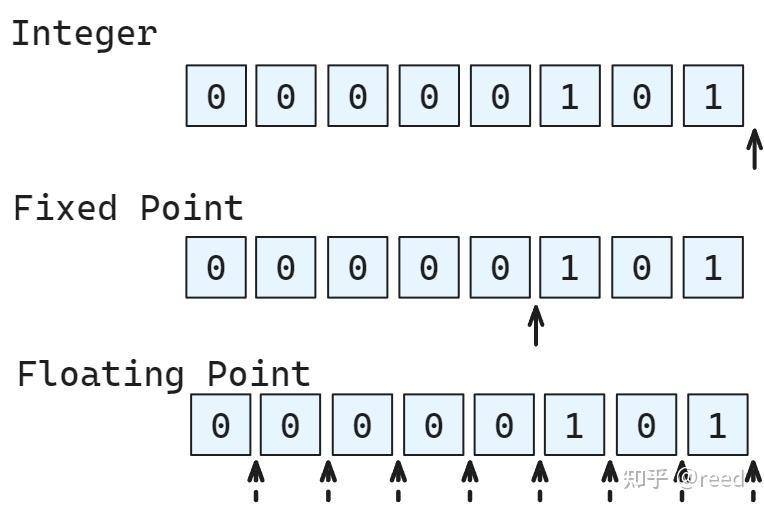
\includegraphics[width=0.9\textwidth]{figures/reed-isa-04-float/fig-01.jpg}
\caption{Figure 1. Integer, Fixed Point and Floating Point Number}
\end{figure}

具体地，如图2所示，对于32bit浮点数，其中1bit为符号bit，0表示正数，1表示负数；8bit的指数位，表示浮点数中点的位置，可以作为无符号的整数来进行取值k，其表示带偏置的指数，k - 127为有偏置的指数位用以实际的浮点数计算，8bit无符号数表示的有效范围为0到255，即[0，255]，减去偏置项127后，指数范围为[-127, 128], 其中全零和全一用以表示特殊的数字，有效的指数为[-126, 127]；指数位之后为尾数位（或者叫有效位）用以表达浮点数中的有效数字，在表示实际数值是会在尾数之前固定的添加一个数字1用以规则化数据（normal），确保数据的第一位是1，从而确保了有效数据的位数为24位。

\begin{figure}[htbp]\centering
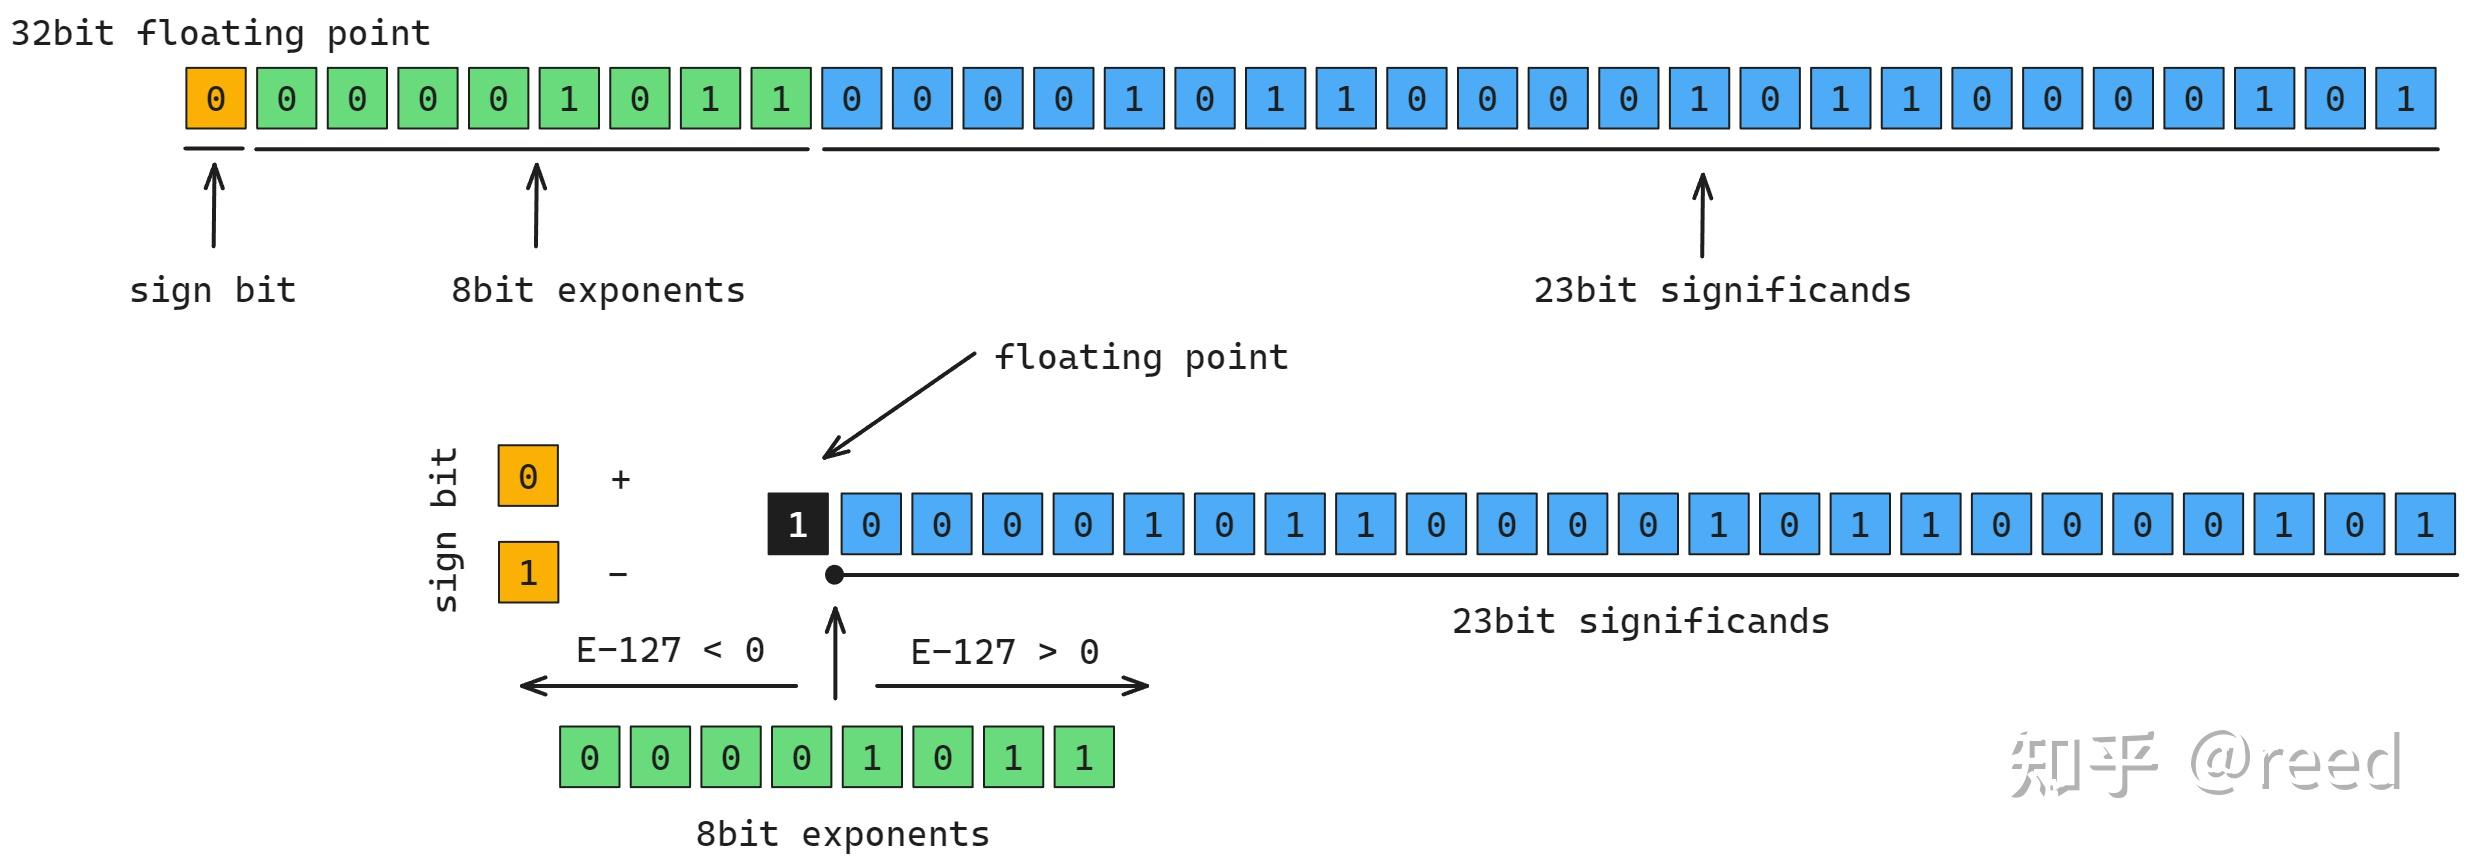
\includegraphics[width=0.9\textwidth]{figures/reed-isa-04-float/fig-02.jpg}
\caption{Figure 2. 32bit floating point bit details}
\end{figure}

浮点数的数值为 $v = (-1)^{sign} \times 2^{(E - 127)} \times 1.S $ ，具体的如图2中，符号位为0，表示v为正数，指数位为b00001011十进制为11，有偏的指数为11-127 = -116，尾数为前面添加1的一个小数，二进制表示为1.00001011000010110000101，十进制表示为1.04313719272613525390625。将指数作用到尾数上后（即将含前缀1的尾数的小数点左移116位），得到的十进制数据为1.25563072223456437348238306129524010182326911326927391629018127862382758763715173699893057346343994140625×10-35。具体的可以参考\url{https://float.exposed/0x05858585}。

\begin{figure}[htbp]\centering
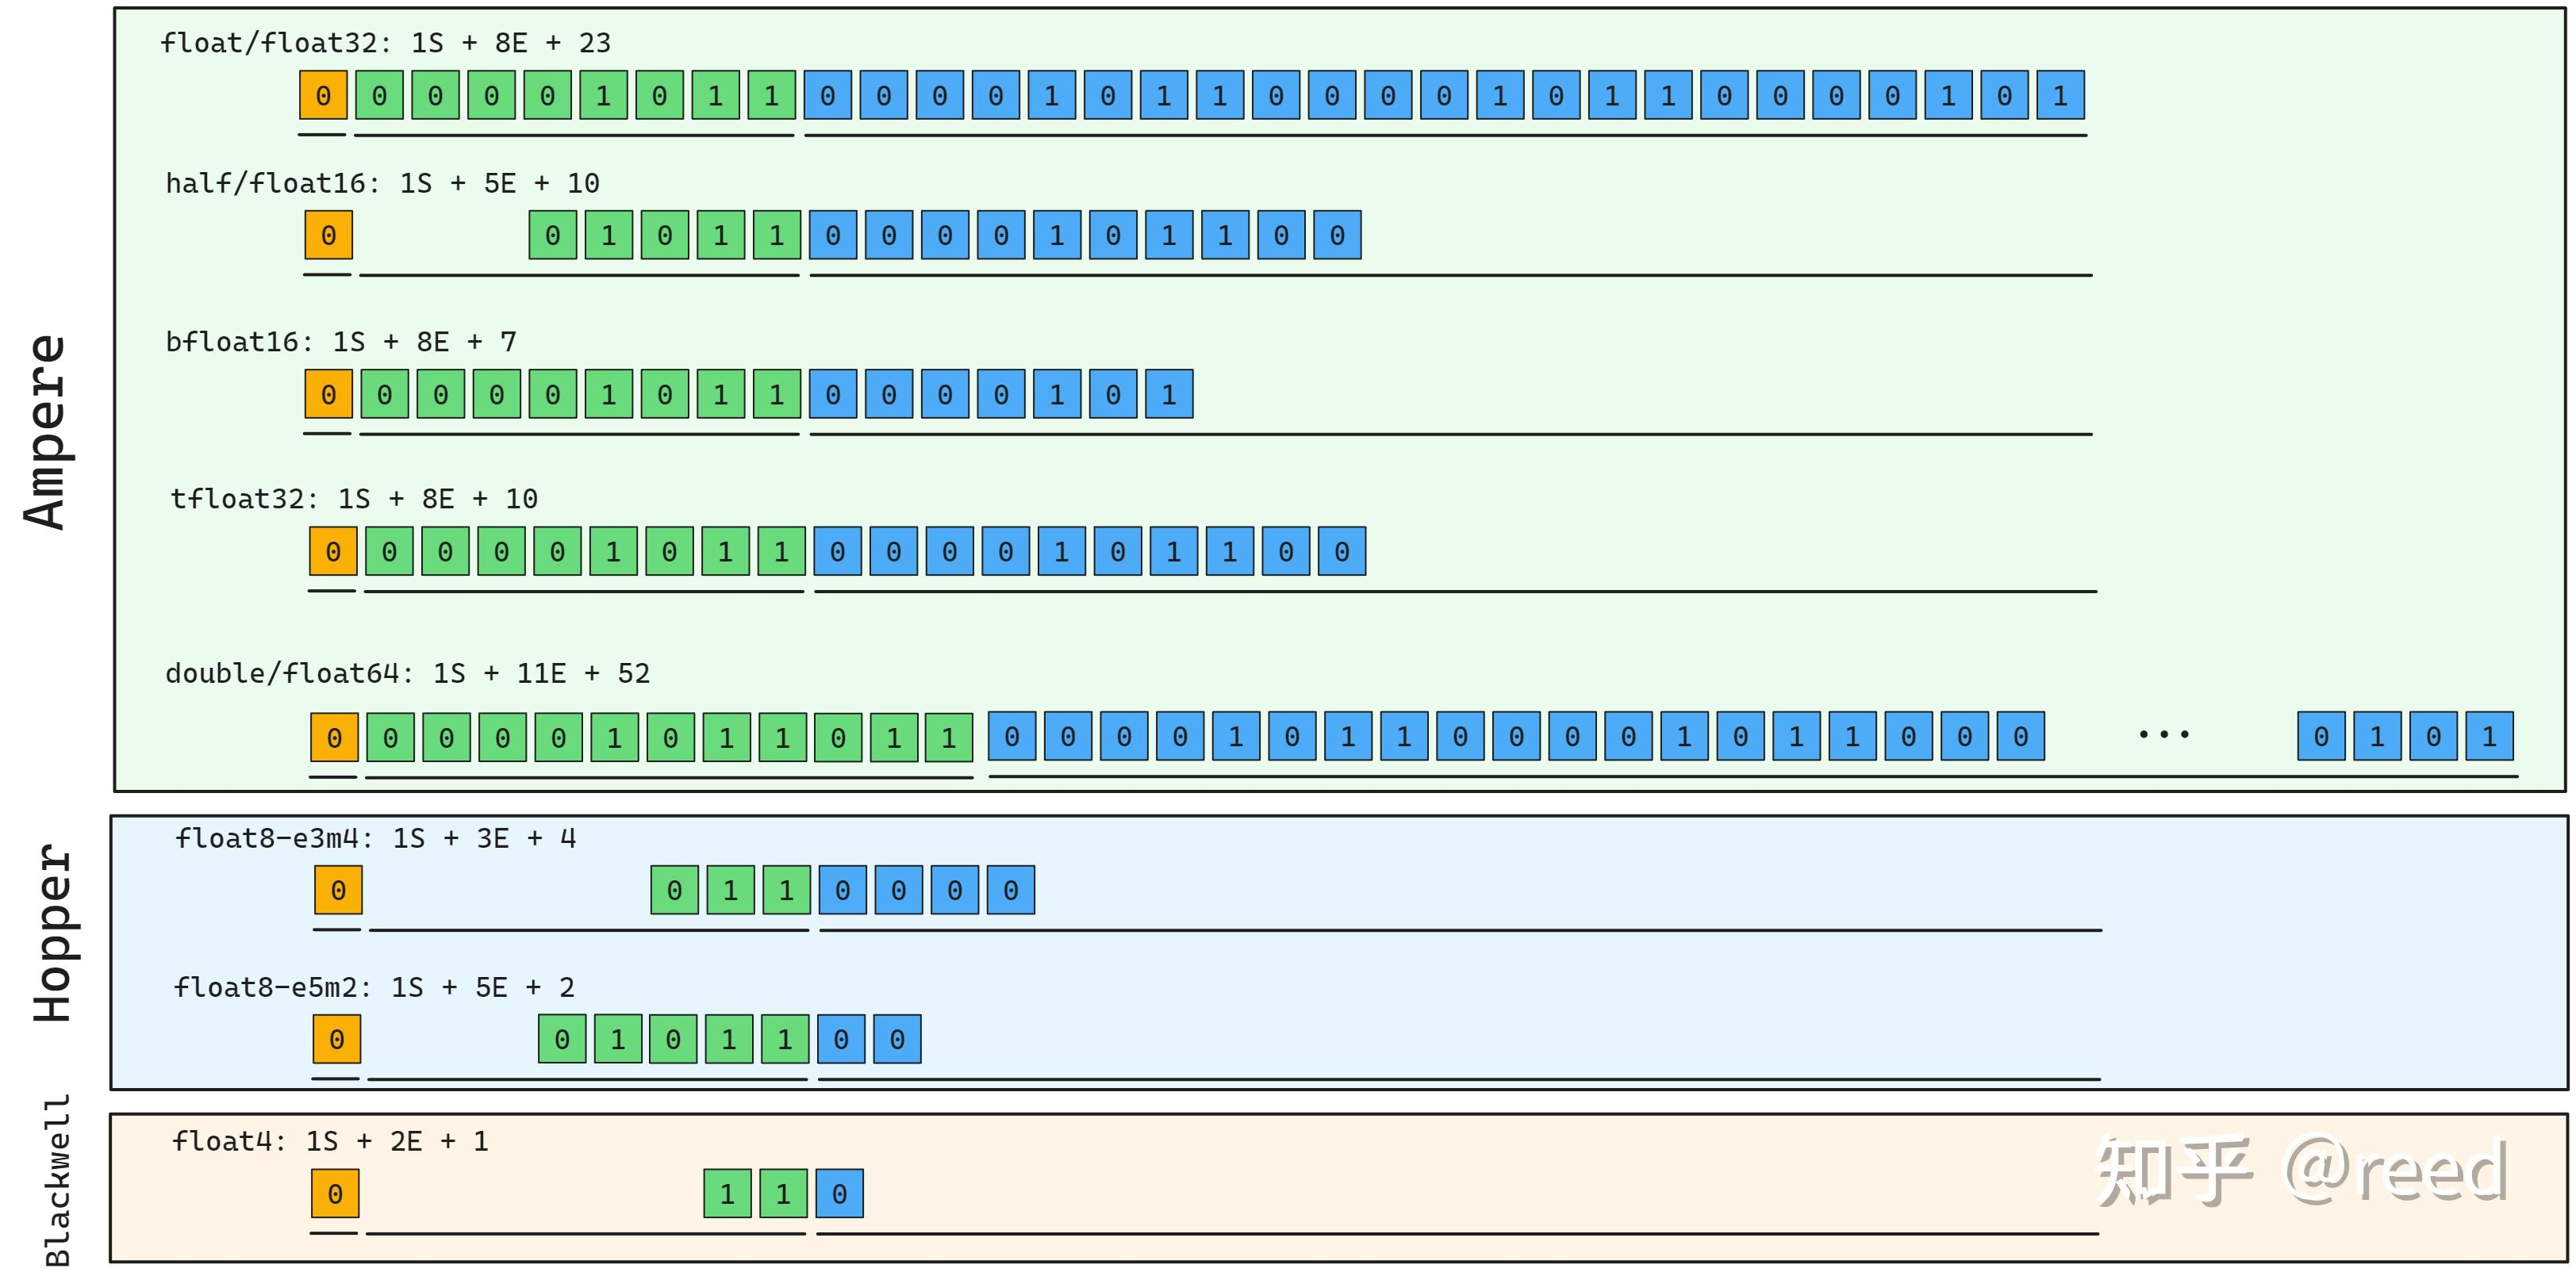
\includegraphics[width=0.9\textwidth]{figures/reed-isa-04-float/fig-03.jpg}
\caption{Figure 3. various floating point with various sign exponents significands bits}
\end{figure}

通过上面的描述我们知道浮点数中通过E指数来调整小数点的位置，通过尾数来表示数据的有效数值。E的容量越大则表示的数据范围约到，尾数的容量越大则表示有效位数越大，数据精度越高。针对不同场景所需求的的数据范围和精度的平衡，Ampere中支持五种类型的浮点数：float32、half（也叫float16）、bfloat16、tfloat32和double精度，hopper中添加了float8类型，根据指数和尾数的多少分为E5M2和E3M4子类型，blackwell架构中添加了fp4类型，具体的各类型的指数和尾数的位数如图3中所示。

\subsection{浮点数的圆整}

由于浮点数是实数的近似表示，IEEE-745标准在定义浮点数上的的四则运算（加减乘除）时为了获得更高的精度则定义了圆整方案，其中有：向最近圆整，向零圆整，向正无穷圆整（up）和向负无穷圆整（down）。一般情况下，四则运算采用最近圆整其能满足标准约束的ULP误差。将浮点数向整数转换时，应用向正无穷圆整则实际为ceiling函数，向负无穷圆整则为floor函数。在一些高精度除法等计算时，需要对数据做特殊的修正，此时也会使用到特定的圆整方式。

\subsection{浮点数特殊值}

在介绍浮点数的指数表示是，其中全0和全1是被保留的。其中指数全1（尾数非全0）的浮点数被解释为NaN（Not A Number），它是浮点数中一类特殊的数值。如零除以零在数学上是无意义的，但是我们必须能用浮点数表示这种无意义，这时候这个计算结果即可以表示为NaN（有些编程语言则实现为异常，对于GPU而言，作为异步设备计算不产生异常），类似地对负数开平方在实数解空间下也是无意义的，其结果也表示为NaN，还有其他类似的指数等运算也可以产生NaN结果。同时NaN有一定的传递性，如过某个计算中间产生了NaN很容易使得后续的结果也为NaN，如NaN + 1.0 = NaN，NaN x 0.0 = NaN。这也是编程中对浮点数表示不熟悉而容易犯的错误，认为一个未初始化的数据乘以0就一定可以可以得到0。其实不然，因为这个未初始化的数据如果是NaN其结果就不是0了。NaN具体的还可以分为Quiet和Signaling，在此我们不再赘述，有兴趣的可以参考IEEE-754标准的介绍。

当指数全1，尾数为全零时，根据符号位的不正负则定义了正无穷（+infinity）和负无穷（-infinity）。正负无穷也是一种相对特殊的表示，但是定义在这上面的数学计算则满足数学规则，如exp(-infinity) = 0。

恰当的使用NaN 和 +Infinity，-Infintiy可以简化和unify一些数学计算而避免一些分支结构。

\subsection{浮点数的denormal}

前文提到针对尾数表示会在前面固定的添加一个1（规则化，normal）确保了数据有效位数为24位，对于E指数为全0时，这时在计算尾数时不再添加这个固定的1，那么尾数的表示可能包含0开头的数据，从而减少了数据的有效位数，这样的数据称为为非规则/正常浮点数（denormal或者subnormal），同时全零的E指数记为 $2^{-126}$ （而非 $2^{-127}$ ）,这样其可以表示较小的0附近比normal数更小的浮点数，加密了0附近的点的数据表示，对于0附近的绝对值特别小的数据能更好的表示。

\begin{figure}[htbp]\centering
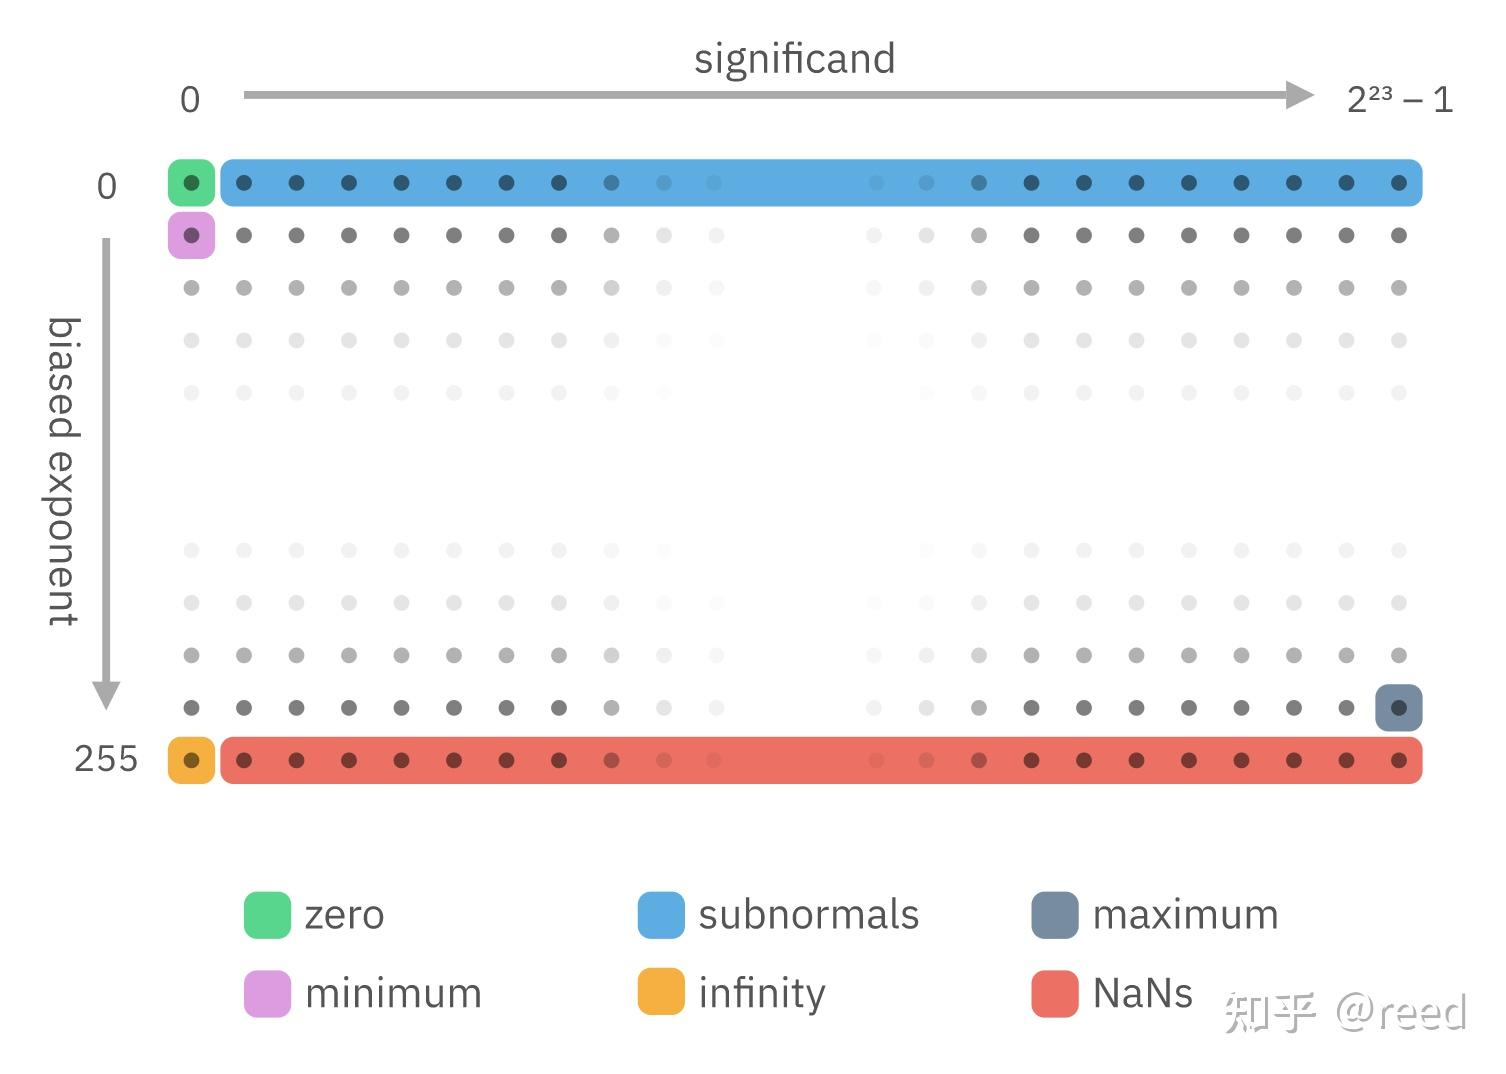
\includegraphics[width=0.9\textwidth]{figures/reed-isa-04-float/fig-04.jpg}
\caption{Figure 4. All the special values of floating point(引用自参考1)}
\end{figure}

图4展示了浮点数中的0，normal数，subnormals，无穷和NaN时指数和尾数的情况。

\section{NVidia GPU浮点运算指令}

\subsection{加法和乘法}

NVidia GPU上实现了IEEE-754标准的加减乘指令和不同的圆整类型，具体地， 加法（FADD = Float Add）和乘法（FMUL = Float MULtiply）指令如下，可以实现float32数据类型的加法和乘法，同时采用默认的Nearest圆整方式，对于double精度，则有DADD(Double Add)和DMUL(Double MULtiply)；

\begin{lstlisting}
FADD R0 R1 R2;     // R0 = R1 + R2  with round to NEAREST
FADD.RZ R0 R1 R2;  // R0 = R1 + R2 with round to ZERO
FADD.RP R0 R1 R2;  // R0 = R1 + R2 with round to POSITIVE(+Infinity)
FADD.RM R0 R1 R2;  // R0 = R1 + R2 with round to MINUS(-Infinity)
FMUL R0 R1 R2;     // R0 = R1 * R2 with round to NEAREST
FMUL.RZ R0 R1 R2;  // R0 = R1 * R2 with round to ZERO
FMUL.RP R0 R1 R2;  // R0 = R1 * R2 with round to POSITIVE(+Infinity)
FMUL.RM R0 R1 R2;  // R0 = R1 * R2 with round to MINUS(-Infinity)

DADD R0 R2 R4;     // R0.64 = R2.64 + R4.64 with round to NEAREST
DADD.RZ R0 R2 R4;  // R0.64 = R2.64 + R4.64 with round to ZERO
DADD.RP R0 R2 R4;  // R0.64 = R2.64 + R4.64 with round to POSITIVE(+Infinity)
DADD.RM R0 R2 R4;  // R0.64 = R2.64 + R4.64 with round to MINUS(-Infinity)
DMUL R0 R2 R4;     // R0.64 = R2.64 * R4.64 with round to NEAREST
DMUL.RZ R0 R2 R4;  // R0.64 = R2.64 * R4.64 with round to ZERO
DMUL.RP R0 R2 R4;  // R0.64 = R2.64 * R4.64 with round to POSITIVE(+Infinity)
DMUL.RM R0 R2 R4;  // R0.64 = R2.64 * R4.64 with round to MINUS(-Infinity)
\end{lstlisting}

对于忽略denormal数据的处理也有对应的modifier（FTZ = flush to ZERO）等

\begin{lstlisting}
FMUL.FTZ R3, R4, R5 ;
\end{lstlisting}

\subsection{乘加FMA（Fused Multiply Add）}

对于乘加运算而言，可以采用两条指令实现，如上面提到的FMUL，然后对乘法的结果调用FADD进行累加，IEEE-754-2008标准提出了FMA的计算标准（Fused Multiply Add）,即可以一条指令完成d = a x b + c的运算，同时中间计算结果的精度是无限精度的，只在最后环节进行圆整操作，其可以提供相较于FMUL + FADD组合指令更高的精度。同时FMA指令的latency和FMUL或FADD是一样的，所以单条FMA指令的是FADD和或FADD吞吐的两倍，具体地，单精度浮点指令为FFMA（Float Fused Multiply Add）,双精度浮点指令为DFMA（Double Fused Multiply Add）它们各自的不同圆整Modifier如下，

\begin{lstlisting}
FFMA R0, R1, R2, R3;  // R0 = R1 * R2 + R3 with round to NEAREST
FFMA.RZ R0, R1, R2, R3;  // R0 = R1 * R2 + R3 with round to ZERO
FFMA RP R0, R1, R2, R3;  // R0 = R1 * R2 + R3 with round to POSITIVE
FFMA.RM R0, R1, R2, R3;  // R0 = R1 * R2 + R3 with round to MINUS

DFMA R0, R2, R4, R6;  // R0 = R2 * R4 + R6 with round to NEAREST
DFMA.RZ R0, R2, R4, R6;  // R0 = R2 * R4 + R6 with round to ZERO
DFMA RP R0, R2, R4, R6;  // R0 = R2 * R4 + R6 with round to POSITIVE
DFMA.RM R0, R2, R4, R6;  // R0 = R2 * R4 + R6 with round to MINUS
\end{lstlisting}

\subsection{随路取负和绝对值}

对于减法而言，NVidia的指令集架构中并没有独立的减法指令，而是在FADD中随路对数据取负实现，即d = a - b可以写做 d = a + (-b)，同时FADD指令中随路做对b的取负操作：

\begin{lstlisting}
FADD R0 R1 -R2;     // R0 = R1 - R2  with round to NEAREST
FADD.RZ R0 R1 -R2;  // R0 = R1 - R2 with round to ZERO
FADD.RP R0 R1 -R2;  // R0 = R1 - R2 with round to POSITIVE(+Infinity)
FADD.RM R0 R1 -R2;  // R0 = R1 - R2 with round to MINUS(-Infinity)
\end{lstlisting}

如此在FADD指令上附加对操作数取负能力，单个指令即可以实现浮点数的加法和减法功能，并且圆整能力保持不变。除了对第二个操作数取负号，NVidia的浮点运算指令集基本上可以实现对任意操作数取负。形如 $d = \pm a \pm \pm b$ ， $d = \pm a \times \pm b$ ， $d = \pm a \times \pm b   \pm c$ 的形式的操作都可以通过FADD、FMUL、FFMA指令随路对操作数取负而单指令完成。甚至NVidia指令集中没直接提供取负的指令，而是通过 d = -d - 0来unify的实现；除了对操作数随路取负，这些浮点指令也可以随路取绝对值操作。如\lstinline|d = abs(a) * abs(b) - abs(c);|可以通过单条FMA指令实现，如下

\begin{lstlisting}
FFMA R7, |R0|, |R7|, -|R6|;
\end{lstlisting}

\subsection{低精度浮点指令}

half、bfloat16是NVidia提供的16bit的浮点数类型，连续的两个16bit数据可以合并成一个32bit的数据（寄存器宽度），该连续的两个half数形成packed类型half2 和 bfloat162类型。因为寄存器宽度是32bit的，所以NVidia的计算指令是针对packed类型而提供的，即便是操作单个half数，也会使用针对packed类型的指令，只是会在操作数上做重复和选择。具体的针对packed half即half2，提供了加法、乘法和乘加指令（HADD2，HMUL2，HFMA2.MMA）,这些指令就不再提供不同的round mode（只有round nearest），而是提供了如饱（SAT，最终结果截断到[0.0, 1.0]）和整流（RELU）的Modifier，同时该指令也提供了随路abs和取负能力。对于packed bfloat16 即bfloat162，没有提供ADD和MUL指令，只提供了\lstinline|HFMA2.BF16_V2|指令，加法乘法等都是使用该FMA实现的，同时该指令支持必要的随路取负和abs能力，modifier方面不如half2类型支持的丰富，只提供了RELU能力。

\begin{lstlisting}
HADD2 R7, R0, R7;
HMUL2 R7, R0, R7;
HADD2.SAT R7, R0, R7;
HMUL2.SAT R7, R0, R7;

HFMA2.MMA R7, R0, R7, R6;
HFMA2.MMA.SAT R7, R0, R7, R6;
HFMA2.MMA.RELU R7, R0, R7, R6;
HADD2 R7, |R2|, -RZ.H0_H0;
HADD2 R7, -R2, -RZ.H0_H0;
HADD2 R7, R0, -R7;

HFMA2.BF16_V2 R7, -RZ.H0_H0, RZ.H0_H0, |R2|;
HFMA2.BF16_V2 R7, R0, 1, 1, R7;
HFMA2.BF16_V2 R7, R0, R7, R6;
HFMA2.BF16_V2.RELU R7, R0, R7, R6;
HFMA2.BF16_V2 R7, R0, R7, -RZ.H0_H0;
HFMA2.BF16_V2 R7, -RZ.H0_H0, RZ.H0_H0, -R2;
HFMA2.BF16_V2 R7, R7, -1, -1, R0;
\end{lstlisting}

\subsection{类型转换}

对于类型转换方面各个类型相互转换的指令如下表格，有些类型直接没有单指令转换的能力，需要借助中间类型类实现，在表格中表现为Multi-Instr(多条指令)

\begin{table}[htbp]
\centering
\begin{tabular}{lllll}
\toprule
转换成-\textgreater{} & float64 & float32 & half & bfloat16 \\
\midrule
float64 & / & F2F.F32.F64 & F2F.F16.F64 & Multi-Instr \\
float32 & F2F.F64.F32 & / & F2FP.PACK\_AB & F2FP.BF16.PACK\_AB \\
half & Multi-Instr & HADD2.F32 & / & NA \\
bfloat16 & Multi-Instr & PRMT & NA & / \\
\bottomrule
\end{tabular}
\end{table}

\subsection{超越函数}

对于浮点数的运算，还有一些特殊的函数，如exp指数，log函数，三角函数（sin、cos等），倒数rcp，平方根sqrt等，这些函数在NVidia指令集架构中是利用特殊函数单元实现（SFU = special function unit），其底层实现是将这些函数分段然后在某一个小段内使用二次函数进行逼近实现（y = ax\textasciicircum{}2 + bx + c），对于不同区间段通过提供不同的a，b，c系数则可以产生相对高精度的结果。也就是说这类特殊函数是通过查表得到系数a/b/c，然后利用二次函数得到最终结果。常见的指令如

\begin{lstlisting}
MUFU.EX2 R7, R6 ;
MUFU.SIN R7, R7 ;
MUFU.COS R7, R7 ;
MUFU.LG2 R7, R0 ;
MUFU.RCP R7, R6 ;
MUFU.RSQ R5, R2 ;
MUFU.SQRT R7, R13 ;
MUFU.TANH R11, R4 ;
\end{lstlisting}

这些函数的精度都是偏低的，对于高精度的需求NVidia NVCC编译器会通过软件的形式对上面结果进行修正，得到更高精度的结果。如果我们对上述计算要求的精度不高可以使用这些函数的快速版本，一般是在函数前加\lstinline|__|前缀，如\lstinline|sinf()|的快速版本\lstinline|__sinf()|。也可以在编译选项中启用\lstinline|use_fast_math|选项来全局使能。

\subsection{除法}

前面介绍了四则运算中的加法、减法、乘法（以及融合的乘加运算），对于除法运算，NVidia指令集中没有提供满足IEEE标准的除法指令，而是通过低精度的特殊函数单元提供的MUFU.RCP倒数能力结合泰勒展开利用FADD、FMUL、FFMA指令进行高阶修正得到，这些高阶修正算法可以通过分析SASS指令得到，如normal数的除法的5阶Taylor修正大概如下

\begin{lstlisting}
MUFU.RCP R8, R5 ;                                   /* 0x0000000500087308 */                                                                                      /* 0x000e220000001000 */
FADD.FTZ R10, -R5, -RZ ;                            /* 0x800000ff050a7221 */
FFMA R3, R8, R10, 1 ;                               /* 0x3f80000008037423 */
FFMA R12, R8, R3, R8 ;                              /* 0x00000003080c7223 */
FFMA R3, R7, R12, RZ ;                              /* 0x0000000c07037223 */
FFMA R8, R10, R3, R7 ;                              /* 0x000000030a087223 */
FFMA R11, R12, R8, R3 ;                             /* 0x000000080c0b7223 */
FFMA R7, R10, R11, R7 ;                             /* 0x0000000b0a077223 */
FFMA R3, R12, R7, R11 ;                             /* 0x000000070c037223 */
\end{lstlisting}

除了前面的计算类指令外，浮点数还有相关的控制流，比较大小，Normal数判断，取整等，它们共同协作完成浮点数相关的计算任务

\begin{lstlisting}
FSETP
FMNMX
FCHK
FRND  FRND.CEIL  FRND.F16.FLOOR  FRND.F64.FLOOR  FRND.FLOOR
\end{lstlisting}

\section{总结}

本文回顾了浮点数的表示和圆整等基础信息，介绍了NVidia GPU指令集架构中的浮点数的相关运算，继而介绍了浮点相关的加法、乘法、乘加指令和特殊函数对浮点数的操作，以及随路的abs能力和取负能力，同时介绍了各种数据类型直接的相互转换指令，了解这些指令能够使我们更清晰的了解硬件对浮点数计算的支持情况，指导我们对算法的设计和数据类型的选择（如FFMA替换FMUL + FADD，HALF2 packed类型替换单元素类型）。

\section{参考}

Exposing Floating Point – Bartosz Ciechanowski\footnote{\url{https://ciechanow.ski/exposing-floating-point/}}

\url{https://ieeexplore.ieee.org/xpl/conhome/1000125/all-proceedings}

\url{https://iremi.univ-reunion.fr/IMG/pdf/ieee-754-2008.pdf}

\url{https://web.ece.ucsb.edu/~parhami/pubs_folder/parh02-arith-encycl-infosys.pdf}

\url{https://en.wikipedia.org/wiki/Floating-point_arithmetic}

\url{https://docs.oracle.com/cd/E19957-01/800-7895/800-7895.pdf}

CUDA Toolkit Documentation\footnote{\url{https://docs.nvidia.com/cuda/cuda-math-api/group__CUDA__MATH__INTRINSIC__SINGLE.html}}
